\clearpage\chapter{The Translation Model}

Modern compilers seldom produce machine code directly. They translate
a program into a form closer to machine code than the source language
and depend on other tools to finish the translation. If the compiler
produces an object module, it depends on a linker and a loader to
produce executable code. If the compiler produces assembly language,
it also depends on an assembler. A trend among compilers
produced in research environments has been to produce C code
[.cbook,ansi-c.], adding a C compiler to the list of tools required to
finish the translation to machine code [Andrews88, Ramakrishnan, Bartlett
89, Yuasa,Stroustrup,yacc,lex.]. The Icon compiler takes this approach
and generates C code.


There are several advantages to compiling a language into C. Low-level
problems such as register allocation and the selection and
optimization of machine instructions are handled by the C compiler. As
long as these problems are outside the scope of the research addressed
by the compiler, it is both reasonable and effective to allow another
compiler to deal with them. In general, it is easier to generate code
in a higher-level language, just as it is easier to program in a
higher-level language. As long as the target language lies on a
``nearly direct path'' from the
source language to machine code, this works well. C is closely matched
to most modern machine architectures, so few tangential translations
must be done in generating C code from Icon.


Another advantage of generating C code is that it greatly increases
the portability of the compiler and facilitates cross-compilation. The
popularity of C in recent years has resulted in production-quality C
compilers for most systems.  While the implementation of Icon in C
contains some machine and system dependencies, C's conditional
compilation, macro, and file inclusion facilities make these
dependencies relatively easy to deal with when they arise. These facts
make possible the development of a highly portable Icon compiler,
allowing the compiler's effectiveness to be tested by Icon's large
user community.

\section{Data Representation}

Because the target language is C, Icon data must be represented as C
data. The careful representation of data and variables is important to
the performance of an implementation of a high-level language such as
Icon. In addition, information provided by type inferencing can be
used to optimize these representations. However, such considerations
are largely outside the scope of this current research. For this
reason, the representations used in code produced by this compiler and
the compiler's run-time system are largely unchanged from those of the
Icon interpreter system described in Part I. The interpreter's
run-time system is written in C. Therefore borrowing its data
representations for the compiler system is simple. This choice of
representation means that the run-time system for the compiler could
be adapted directly from the run-time system for the interpreter, and
it allowed the compiler development to concentrate on parts of the
system addressed by this research. In addition, this choice of
representation allows a meaningful comparison of the performance of
compiled code to the performance of interpreted code.


An Icon value is represented by a two-word descriptor (see Section
4.1). The first word, the \textit{d-word}, contains type
information. In the case of a string value, the type is indicated by
zero in a high-order bit in the d-word, and the length of a string is
stored in low-order bits of the d-word. All other types have a one in
that bit and further type information elsewhere in the d-word. The
\textit{v-word} of a descriptor indicates the value. The v-word of the
null value is zero, the v-word of an Icon integer is the corresponding
C integer value, and v-words of other types are pointers to data. A
descriptor is implemented with the following C structure:

\goodbreak
\begin{iconcode}
struct descrip \{\\
\>word dword; /* type field */\\
\>union \{\\
\>\>word integr; /* integer value */\\
\>\>char sptr; /* pointer to character string */\\
\>\>union block bptr; /* pointer to a block */\\
\>\>dptr descptr; /* pointer to a descriptor */\\
\>\} vword;\\
\};\\
\end{iconcode}

\noindent
\texttt{word} is defined to be a C integer type (one that is at least
32-bits long), \texttt{block} is a union of structures implementing
various data types, and \texttt{dptr} is a pointer to
a \texttt{descrip} structure.

\section{Intermediate Results}

While the representation of data in the compiler is the same as in the
interpreter, the method of storing the intermediate results of
expression evaluation is not. Two basic approaches have been used in
language implementations to store intermediate results. A stack-based
approach is simple and dynamic. It requires no pre-analysis of
expressions to allocate storage for the intermediate results, but the
simple rigid protocol allows little room for optimization.  For Icon
there is an additional problem with a stack-based
approach. Goal-directed evaluation extends the lifetime of some
intermediate results, requiring that the top elements of the
evaluation stack be copied at critical points in execution [see Part
I, or UA tr88-31]. In spite of the need for this extra copying, most
previous implementations of Icon have been implemented with an
evaluation stack.

An alternative to using a stack is to pre-allocate a temporary
variable for each intermediate result. In this model, operations take
explicit locations as arguments. Therefore an operation can directly
access program variables as arguments; there is no need to perform the
extra operations of pushing addresses or values on a stack. In
addition, the lifetime of a temporary variable is not determined by a
rigid protocol. The compiler can assign an intermediate result to a
temporary variable over an arbitrary portion of the program,
eliminating the copying needed to preserve a value beyond the lifetime
imposed by a stack-based approach. This compiler uses the
temporary-variable model because it allows more opportunities to
optimize parameter handling, a major goal of this research.


Icon's automatic storage management dictates the use of a garbage
collector in the run-time system. When this garbage collector is
invoked, it must be able to locate all values that may be used later
in the program. In the interpreter system, intermediate values and
local variables are stored on the same stack. The garbage collector
sweeps this stack to locate values. In the compiler, a different
approach is taken to insure that all necessary values are locatable.
Arrays of descriptors are allocated contiguously along with a count of
the number of descriptors in the array. The arrays are chained
together. An array of descriptors may be local to a C function, or it
may be allocated with the malloc library function. The garbage
collector locates values by following the chain and scanning the
descriptors in each array. These descriptors are referred to as
\textit{tended} descriptors.

\section{Executable Code}

Even more important than where intermediate results are stored is how
they are computed. Some aspects of Icon expression evaluation are
similar to those of many other languages, but others aspects are
not. Goal-directed evaluation with backtracking poses a particular
challenge when implementing Icon expression evaluation. The Icon
interpreter is based on a virtual machine that includes backtracking,
as are Prolog interpreters based on the Warren Abstract Machine
[.wam.]. While details differ between the Icon and Prolog virtual
machines, their implementation of control backtracking is based on the
same abstract data structures and state variables. Such a virtual
machine contains a stack of procedure frames, but the stack is
maintained differently from that of a virtual machine that does not
implement goal-directed evaluation.

The difference manifests itself when a procedure produces a result,
but has alternate results that it can produce in the event of
backtracking. When this occurs, the frame for the procedure remains on
the stack after control returns to the caller of the procedure. This
frame contains the information needed to produce the alternate
results. The left stack in the following diagram shows that procedure
\texttt{f} has called procedure \texttt{g}. The arrows on the left of
the stack represent the \textit{backtracking chain} of procedures that
can produce alternate results. \texttt{btp} points to the head of the
backtracking chain which currently starts further down in the
stack. The arrows on the right represent the call chain of procedures.
\texttt{fp} points to the frame of the currently executing procedure.

\begin{figure}[htb]
{\centering\selectlanguage{english}
%-% 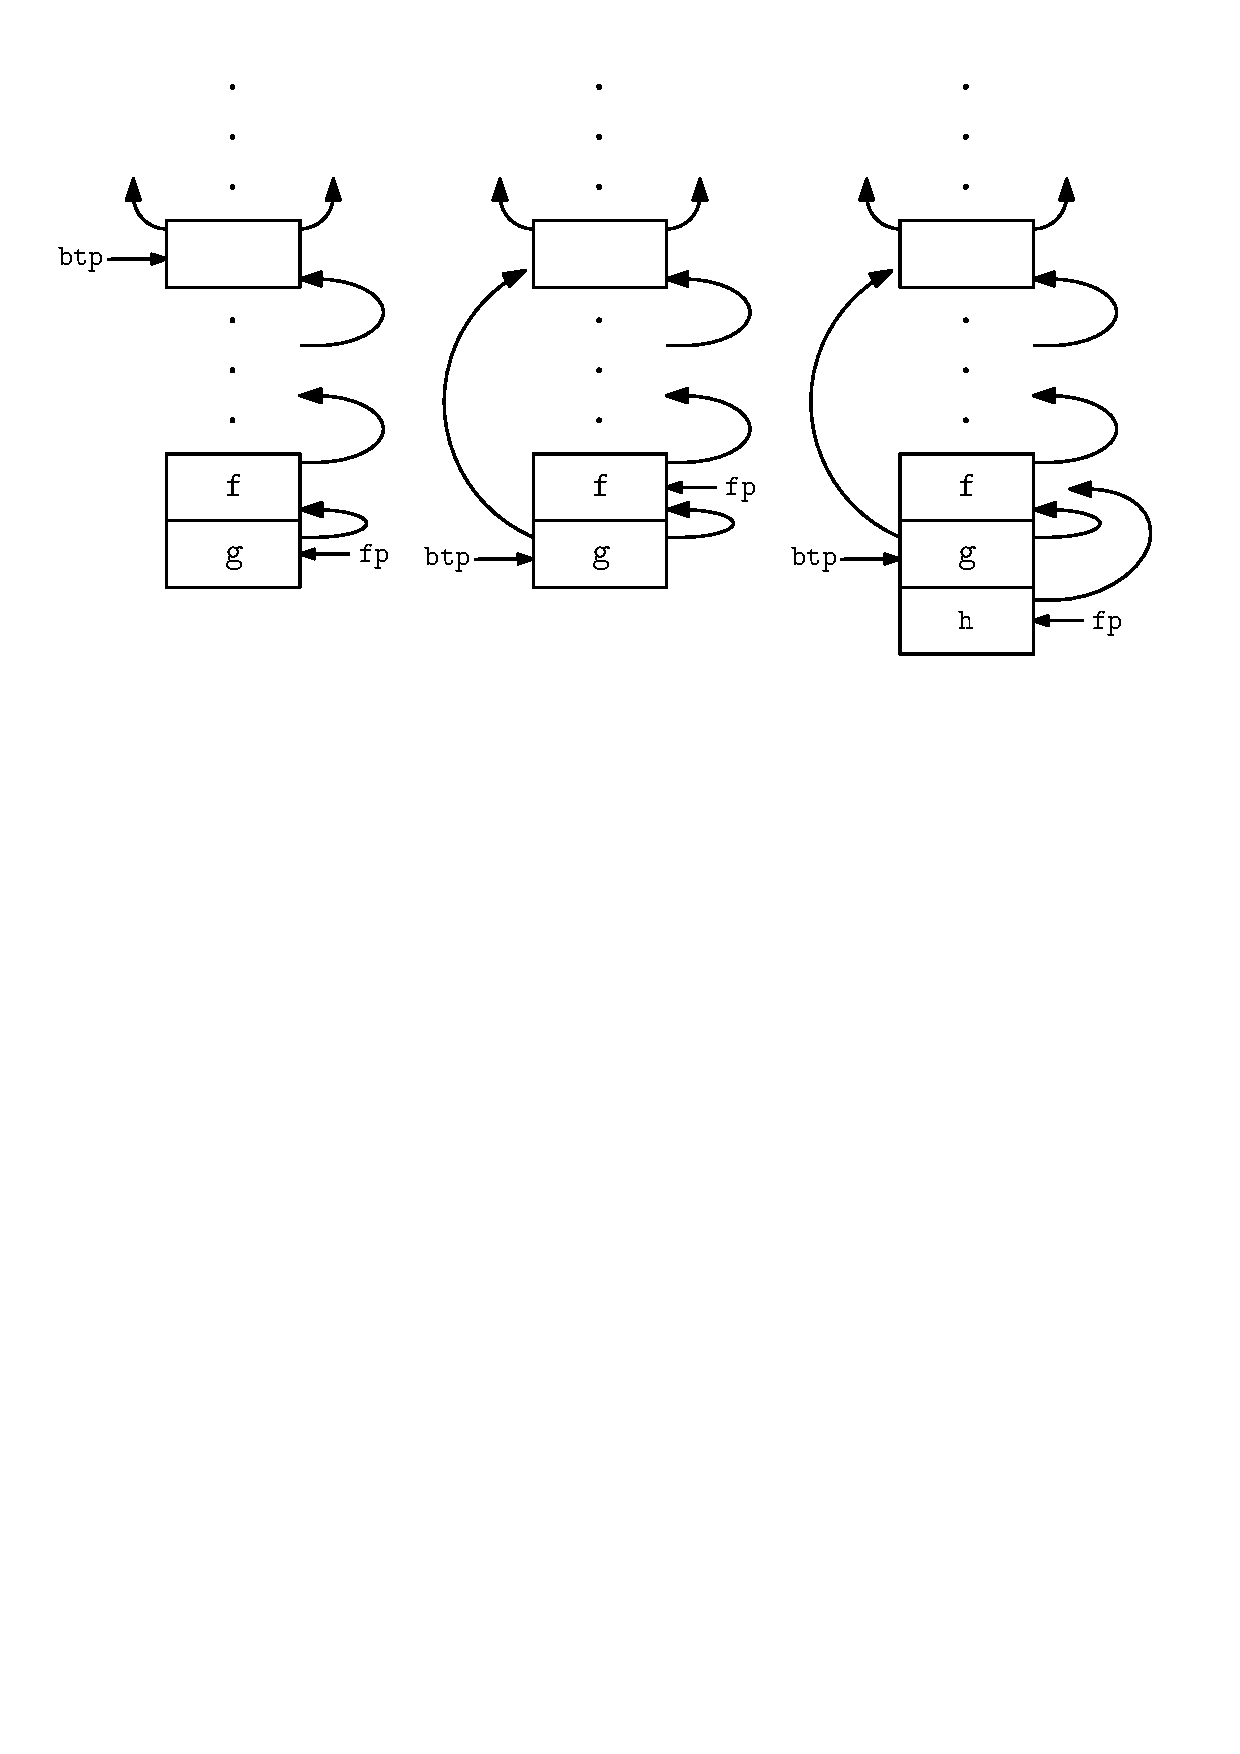
\includegraphics[width=5in]{ib-img/BackTrackingChain.pdf}
%-% 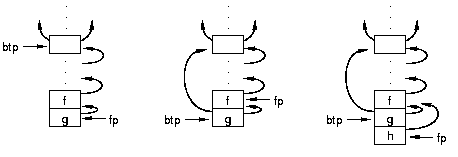
\includegraphics[width=5.0319in,height=1.6346in]{kw/figure2-1.png}

\begin{tikzpicture}[>=latex]
\matrix [thick, nodes={minimum height=4mm, minimum width=12mm, font=\tt}]
{
% uppper dots
% The matrix column sep option appears to add an extra separation after the final column
% so we use the first row to define the column separations
\node{.}; &[3.2cm] \node{.}; &[3.2cm] \node{.}; \\
\node{.}; & \node{.}; & \node{.}; \\
\node{.}; & \node{.}; & \node{.}; \\

% top row of empty boxes (tl = top left, tm = top middle, tr = top right)
\node (tl) [draw, minimum height=8mm] {}; &
\node (tm) [draw, minimum height=8mm] {}; &
\node (tr) [draw, minimum height=8mm] {};\\

% middle dots
\node{.}; & \node{.}; & \node{.}; \\
\node (mdl) {.}; & \node (mdm) {.}; & \node (mdr) {.}; \\ % mdl = middle dot left etc.
\node{.}; & \node{.}; & \node{.}; \\

% f boxes (left middle and right)
\node (fl) [draw, minimum height=8mm] {f}; & 
\node (fm) [draw, minimum height=8mm] {f}; &
\node (fr) [draw, minimum height=8mm] {f};\\[-0.8pt] % subtract width of a thick line to avoid a very thick line between boxes

% g boxes (left middle and right)
\node (gl) [draw, minimum height=8mm] {g}; &
\node (gm) [draw, minimum height=8mm] {g}; &
\node (gr) [draw, minimum height=8mm] {g}; &\\[-0.8pt]

 % h box (right only)
 & & \node (hr) [draw, minimum height=8mm] {h}; \\
};

% draw connecting arrows between the labelled nodes
\begin{scope}[thick,font=\tt\small]
\foreach \s / \d in {gm/tm, gr/tr} { % draw backtracking chain on the left
   \draw[->] ($(\s.north west) -(0,2mm)$) to [distance=1.2cm, out=155, in=205] ($(\d.south west) +(-1mm,2mm)$);
}
\foreach \s / \d in {gl/fl, gm/fm, gr/fr} { % connect g boxes to f boxes on the right
   \draw[->] ($(\s.north east) -(0,2mm)$) to [distance=1cm, out=0, in=0] ($(\d.south east)+ (0,2mm)$);
}
\foreach \s / \d in {mdl/tl, mdm/tm, mdr/tr} { % connect middle dots and top boxes
   \draw[->] (\s.north east) to [distance=1cm, out=0, in=0] ($(\d.south east)+ (0,2mm)$);
}
\foreach \s / \d in {fl/mdl, fm/mdm, fr/mdr} { %connect f boxes and middle dots
   \draw[->] ($(\s.north east) -(0,2mm)$) to [distance=1cm, out=0, in=0] (\d.south east);
}
\foreach \n in {tl, gm, gr} { % add btp pointers
  \draw ($(\n.west) - (1cm,0)$) node (x) {btp} ;
  \draw[->] (x.east) -- (\n.west);
}
\foreach \n in {gl, fm, hr} { % add fp pointers
  \draw ($(\n.east) + (1cm,0)$) node (x) {fp} ;
  \draw[->] (x.west) -- (\n.east);
}
\foreach \n in {tl,tm,tr} { % add left and right back pointers to top boxes
  \draw[->] ($(\n.north west) - (0,2mm)$) to [out=180, in=270] +(-0.4cm,0.5cm);
  \draw[->] ($(\n.north east) - (0,2mm)$) to [out=0, in=270] +(0.4cm,0.5cm);
}
\draw[->] ($(hr.north east) - (0,2mm)$) to [distance=1.5cm, out=0, in=0] ($(fr.east) + (0.25cm,0)$);
\end{scope}
%\draw[red] (current bounding box.south west) rectangle (current bounding box.north east);
\end{tikzpicture}

\par}
\caption{The backtracking chain}
\end{figure}

Suppose \texttt{g} produces the first of several possible
results. Execution returns to \texttt{f} and \texttt{g}'s frame is
added to the backtracking chain. This is represented by the middle
stack in the diagram. If \texttt{f} then calls \texttt{h}, its
procedure frame is added to the top of the stack as shown in the right
stack in the diagram.

If \texttt{h} produces a result and is not capable of producing more,
execution returns to \texttt{f} and the stack again looks like the one
in the middle of the diagram (the program pointer within \texttt{f} is
different, of course). If \texttt{h} produces a result and is capable
of producing more, execution returns to \texttt{f}, but \texttt{h}'s
frame remains on the stack and is added to the head backtracking
chain, similar to what was done when \texttt{g} produced a result.
If \texttt{h} produces no results, backtracking occurs.  \texttt{h}'s
frame is removed from the stack, execution returns to the
procedure \texttt{g} who's frame is at the head of the backtracking
chain, and \texttt{g}'s frame is removed from the head of the
chain. The stack once again looks like left stack in the diagram
and \texttt{g} proceeds to produce another result.


Traditional languages such as Pascal or C present high-level virtual
machines that contain no notion of backtracking and have no need to
perform low-level stack manipulations. Icon expressions with
goal-directed evaluation cannot be translated directly into such
languages. This is the fundamental problem that must be addressed when
designing a compiler for Icon. O'Bagy presents an elegant solution to
this problem in her dissertation [.tr88-31.]. Her solution is used by
this optimizing compiler as a basis for translating Icon expressions
into C code. The rest of this section contains a brief explanation of
the variation of her approach that is used in the compiler, while
exploring useful ways of viewing the problem. O'Bagy's dissertation
describes how control structures not covered in this discussion can be
implemented using her model.

Formal semantics is one tool that can be used in understanding a
language [.gordon denote,stoy.]. The added complexity caused by Icon's
goal-directed evaluation is reflected in Gudeman's description of Icon
using denotational semantics [.gudeman denotational.]. While
conventional programming languages can be described using one
continuation for each expression, Icon requires two continuations. One
continuation for an expression embodies the rest of the program if the
expression succeeds, while the other embodies the rest of the program
if the expression fails.

The Icon compiler uses the notion of success continuations to
implement goal-directed evaluation. However, these continuations
violate some of the properties traditionally associated with
continuations. A continuation in denotational semantics and in the
language Scheme [.Abelson,[Rees 86].] is a function that never
returns. However, the success continuations produced by the compiler
implement backtracking by returning. In addition, these continuations
implement the rest of the current bounded expression rather than the
rest of the entire program. Note that unlike continuations in Scheme,
these continuations are created at compile time, not at run time. Some
Prolog compilers have been based on a similar continuation-passing
technique [.Nilsson,Ramakrishnan.].

The C language is oriented toward an imperative style of
programming. In order to produce efficient code, the Icon compiler
should not generate an excessive number of function
calls. Specifically, it should avoid creating continuations for every
expression. A more operational view of Icon's semantics and of C's
semantics can be useful in understanding how to accomplish this. An
operation in Icon can succeed or fail. In the view of denotational
semantics, the question of what will be done in each case must be
answered, with the answers taking the form of functions. In an
operational view, the questions can take the form of where to go in
each case. The answers to these questions can be any type of transfer
of control supported by the C language: execute the next sequential
instruction, execute a function, return from a function, or go to a
label.

Most operations in Icon are \textit{monogenic}. That is, they produce
exactly one result, like operations in conventional languages. For
these operations, the compiler can generate code whose execution
simply falls through into the code that implements the subsequent
operation.

\textit{Conditional} operations are more interesting. These operations
either produce a single value or fail. If such an operation succeeds,
execution can fall through into code implementing the subsequent
operation. However, if the operation fails, execution must transfer
elsewhere in the program. This is accomplished by branching to a
\textit{failure label}. If the code for the operation is put in-line,
this is straightforward. However, if the operation (either a built-in
operation or an Icon procedure) is implemented by a separate C
function, the function must notify the caller whether it succeeded or
failed and the caller must effect the appropriate transfer of control.

By convention, C functions produced by the compiler and those
implementing the run-time routines each return a signal (this
convention is violated in some special cases). A signal is an integer
(and is unrelated to Unix signals). If one of these C functions needs
to return an Icon value, it does so through a pointer to a result
location that is passed to it as an argument. Two standard signals are
represented by the manifest constants \texttt{A\_Continue} and
\texttt{A\_Resume}. A return (either an Icon return expression or
the equivalent construct in a built-in operation) is implemented with
code similar to

\goodbreak
\begin{iconcode}
*result = \textit{operation result};\\
return A\_Continue;\\
\end{iconcode}

\noindent Failure is implemented with the code 

\iconline{return A\_Resume; }


\noindent The code implementing the call of an operation consists of
both a C call and signal-handling code.

\goodbreak
\begin{iconcode}
switch (\textit{operation}(\textit{args}, \&result)) \{\\
\>case A\_Continue: break;\\
\>case A\_Resume: goto failure label;\\
\}\\
\end{iconcode}


This code clearly can be simplified. This form is general enough to
handle the more complex signal handling that can arise during code
generation. Simplifying signal handling code is described in Chapter
21.


Generators pose the real challenge in implementing Icon. A generator
includes code that must be executed if subsequent failure occurs. In
addition, a generator, in general, needs to retain state information
between suspending and being resumed. As mentioned above, this is
accomplished by calling a success continuation. The success
continuation contains subsequent operations. If an operation in the
continuation fails, an \texttt{A\_Resume} signal is returned to the generator,
which then executes the appropriate code. The generator retains state
information in local variables. If the generator is implemented as a C
function, a pointer to the continuation is passed to it. Therefore, a
function implementing a generative operation need not know its success
continuation until run time.


Consider the operation \texttt{i to j}. This operation can be
implemented in Icon with a procedure like

\goodbreak
\begin{iconcode}
procedure To(i, j)\\
\>while i <= j do \{\\
\>\>suspend i\\
\>\>i +:= 1\\
\>\}\\
\>fail\\
end\\
\end{iconcode}


It can be implemented by an analogous C function similar to the
following (for simplicity, C ints are used here instead of Icon
values).

\goodbreak
\begin{iconcode}
int to(i, j, result, succ\_cont)\\
\>int i, j;\\
\>int *result;\\
\>int (*succ\_cont)();\\
\{\\
\>int signal;\\
\\
\>while (i <= j) \{\\
\>\>*result = i;\\
\>\>signal = (*succ\_cont)();\\
\>\>if (signal != A\_Resume)\\
\>\>\>return signal;\\
\>\>++i;\\
\>\}\\
\>return A\_Resume;\\
\}\\
\end{iconcode}

\noindent
There is no explicit failure label in this code, but it is possible to
view the code as if an implicit failure label occurs before the \texttt{++i}.


The Icon expression 

\iconline{every write(1 to 3) }

\noindent can be compiled into the following code (for simplicity, the
\texttt{write} function has been translated into \texttt{printf} and
scoping issues for result have been ignored). Note that the \texttt{every}
simply introduces failure.

\goodbreak
\begin{iconcode}
switch (to(1, 3, \&result, sc)) \{ /* standard signal-handling code */\\
\>\textit{...}\\
\}\\
\\
int sc() \{\\
\>printf("\%d{\textbackslash}n", result);\\
\>return A\_Resume;\\
\}\\
\end{iconcode}


The final aspect of Icon expression evaluation that must be dealt with
is that of bounded expressions. Once execution leaves a bounded
expression, that expression cannot be resumed. At this point, the
state of the computation with respect to backtracking looks as it did
when execution entered the bounded expression. This means that, in
generated code, where to go on failure (either by branching to an
explicit failure label or by returning an \texttt{A\_Resume} signal)
must be the same. However, this failure action is only correct in the
C function containing the start of the code for the bounded
expression. If a function suspended by calling a success continuation,
execution is no longer in that original C function. To accommodate
this restoration of failure action, execution must return to that
original function.

This is accomplished by setting up a \textit{bounding label} in the
original C function and allocating a signal that corresponds to the
label. When the end of the bounded expression is reached, the signal
for the bounding label is returned. When the signal reaches the
function containing the label, it is converted into
a \texttt{goto}. It can be determined statically which calls must
convert which signals. Note that if the bounded expression ends in the
original C function, the ``return signal'' is already in the context
of the label. In this case, it is immediately transformed into
a \texttt{goto} by the compiler, and there is no real signal handling.


Consider the Icon expression 

\goodbreak
\begin{iconcode}
move(1);\\
\>\textit{...}\\
\end{iconcode}

\noindent
The \texttt{move} function suspends and the C function implementing it
needs a success continuation. In this case, \texttt{move} is called in
a bounded context, so the success continuation must return execution
to the function that called \texttt{move}. The continuation makes use
of the fact that, like the C function for \texttt{to}, the one
for \texttt{move} only intercepts \texttt{A\_Resume} signals and
passes all other signals on to its caller.

This expression can be implemented with code similar to the
following. There are two possible signals that might be returned.
\texttt{move} itself might produce an \texttt{A\_Resume} signal or it
might pass along the bounding signal from the success continuation.
Note that for a compound expression, both the bounding label and the
failure label are the same. In general, this is not true. In this
context, the result of \texttt{move(1)} is discarded. The variable
\texttt{trashcan} receives this value; it is never read.

\goodbreak
\begin{iconcode}
\>switch (move(1, \&trashcan, sc)) \{\\
\>\>case 1:\\
\>\>\>goto L1;\\
\>\>case A\_Resume:\\
\>\>\>goto L1;\\
\>\}\\
L1: /* bounding label \& failure label */\\
\>\textit{...}\\
\end{iconcode}
\goodbreak
\begin{iconcode}
int sc() \{\\
\>return 1; /* bound signal */\\
\}\\
\end{iconcode}

\noindent
{\sffamily
Calling Conventions}


This discussion has touched on the subject of calling conventions for
run-time routines. In Icon, it is, in general, impossible to know
until run time what an invocation is invoking. This is handled in the
compiler with a standard calling convention for the C functions
implementing operations and procedures. This calling convention allows
a C function to be called without knowing anything about the operation
it implements.

A function conforming to the standard calling convention has four
parameters. These parameters are, in order of appearance, the number
of Icon arguments (a C int), a pointer to the beginning of an array of
descriptors holding the Icon arguments, a pointer to the descriptor
used as the Icon result location, and a success continuation to use
for suspension. The function itself is responsible for any argument
conversions including dereferencing, and for argument list
adjustment. As explained above, the function returns an integer
signal. The function is allowed to return the signals
\texttt{A\_Resume}, \texttt{A\_Continue}, and any signals returned by
the success continuation. It may ignore the success continuation if it
does not suspend. The function may be passed a null continuation. This
indicates that the function will not be resumed. In this case, suspend
acts like a simple return, passing back the signal \texttt{A\_Continue}
(this is not shown in the examples). The outline of a
standard-conforming function is

\goodbreak
\begin{iconcode}
int \textit{function-name}(nargs, args, result, succ\_cont)\\
int nargs; dptr args; dptr result;\\
continuation succ\_cont;\\
\{\\
\>\ ...\\
\}\\
\end{iconcode}

\noindent
\texttt{continuation} is defined to be a pointer to a function taking
no arguments and returning an integer.

Later sections of this dissertation describe the code generation
process in more detail and describe optimizations of various parts of
the code including parameter passing, continuations, signal handling,
and branching.


\bigskip

\clearpage
\bigskip
